\documentclass[11pt,a4paper]{article}
\usepackage[margin=2.2cm]{geometry}
\usepackage[T1]{fontenc}
\usepackage{lmodern}
\usepackage{graphicx}
\usepackage{booktabs}
\usepackage{tabularx}
\usepackage{float}
\usepackage[hidelinks]{hyperref}
\setlength{\parskip}{4pt}
\setlength{\parindent}{0pt}
% small captions with a bold label (without the caption package)
\makeatletter
\long\def\@makecaption#1#2{\vskip 4pt{\small\textbf{#1.} #2\par}\vskip 2pt}
\makeatother

\title{From seasonal to extreme flooding in South Sudan:\\drivers, upstream early warning and ADM3 prioritisation}
\author{Group 22 --- JBG060 Capstone Data Challenge\\Eindhoven University of Technology \& Zero Hunger Lab}
\date{}

\begin{document}
\maketitle

% ---------------------------------------------------------------------------------------------
\section{Context / Problem Background / Motivation of Analysis}
Seasonal flooding is part of life in South Sudan: rivers and the Sudd wetland rise every rainy season, and
agro-pastoral livelihoods depend on it. Since 2020 this pattern has broken down. Large parts of Unity and Jonglei have
stayed flooded for years, displacing hundreds of thousands of people and deepening food insecurity.
Humanitarian actors such as WFP increasingly fund \emph{anticipatory action}, releasing money and stock before a
forecast shock; this needs early recognition of extreme floods and knowledge of where hazard meets vulnerable
people. We therefore ask what turns normal flooding into extreme flooding, whether it can be seen coming
upstream, and where action should go first.

% ---------------------------------------------------------------------------------------------
\section{Business and Data Understanding}
\textbf{Stakeholders.}
\begin{itemize}\setlength\itemsep{0pt}
\item WFP and donors need lead time and ADM3 rankings to trigger financing.
\item Technical clusters and national authorities need transparent, justifiable indices.
\item Agro-pastoralists need warnings they can act on.
\end{itemize}

\textbf{Background.} The White Nile leaves Lake Victoria, passes Lakes Kyoga and Albert (Uganda) and enters the Sudd;
the Sobat brings water from the Ethiopian highlands. In 1961--64 a sharp rise of Lake Victoria made the Sudd about 2.5
times larger for years \cite{sutcliffe2018,sutcliffe1999}. East African rain is strongly modulated by the Indian
Ocean Dipole (IOD) \cite{saji1999}.

\textbf{Data and concepts.} Table~\ref{tab:data} lists the stakeholder data and the open data we added for a longer record and independent checks.
\begin{itemize}\setlength\itemsep{0pt}
\item The flood product labels each flooded pixel \emph{recurring} (flooded in at least about a third of years) or
\emph{unusual}. We use unusual flooding as the signature of an extreme flood.
\item An \emph{anomaly} is the deviation from the normal value for that week of the year.
\item \emph{Lead time} is how far ahead a warning is issued.
\end{itemize}

\textbf{Data understanding.} Four findings shaped the approach (Figure~\ref{fig:context}):
\begin{itemize}\setlength\itemsep{0pt}
\item The Lake Victoria and Kyoga files end in 2002, which left Lake Albert as the only upstream gauge until we
added NASA G-REALM.
\item DFO discharge at Malakal falls while the Sudd floods, which points to satellite saturation.
\item Flood masks before 2003 have too few observation days.
\item Unusual flooding in the Sudd grew more than thirty-fold after 2020, while Lake Albert stood 2--3\,m above
normal.
\end{itemize}

\begin{table}[H]
\centering\small
\caption{Data sources (2003--2025 unless stated).}
\label{tab:data}
\begin{tabularx}{\textwidth}{@{}lXl@{}}
\toprule
Source & Use & Origin\\
\midrule
MODIS/VIIRS flood masks (MCDWD) & target: recurring/unusual flood area & stakeholder\\
ERA5 rain and runoff \cite{hersbach2020}, AgERA5 evaporation & regional rainfall and water balance & stakeholder\\
DAHITI Lake Albert altimetry & upstream water level & stakeholder\\
DFO discharge (Malakal, SW Ethiopia) & local river flow (flagged) & stakeholder\\
Payams, population, ICPAC cattle, county IPC & exposure and vulnerability (SQ3) & stakeholder/team\\
NASA G-REALM lake levels (1992--2026) & Lake Victoria/Kyoga after 2002 & added\\
JRC Global Surface Water (1984--2021) \cite{pekel2016} & longer Sudd water record & added\\
NOAA Indian Ocean Dipole index & climate driver & added\\
GLIDE / Dartmouth Flood Observatory & documented flood events & added\\
\bottomrule
\end{tabularx}
\end{table}

\begin{figure}[H]
\centering
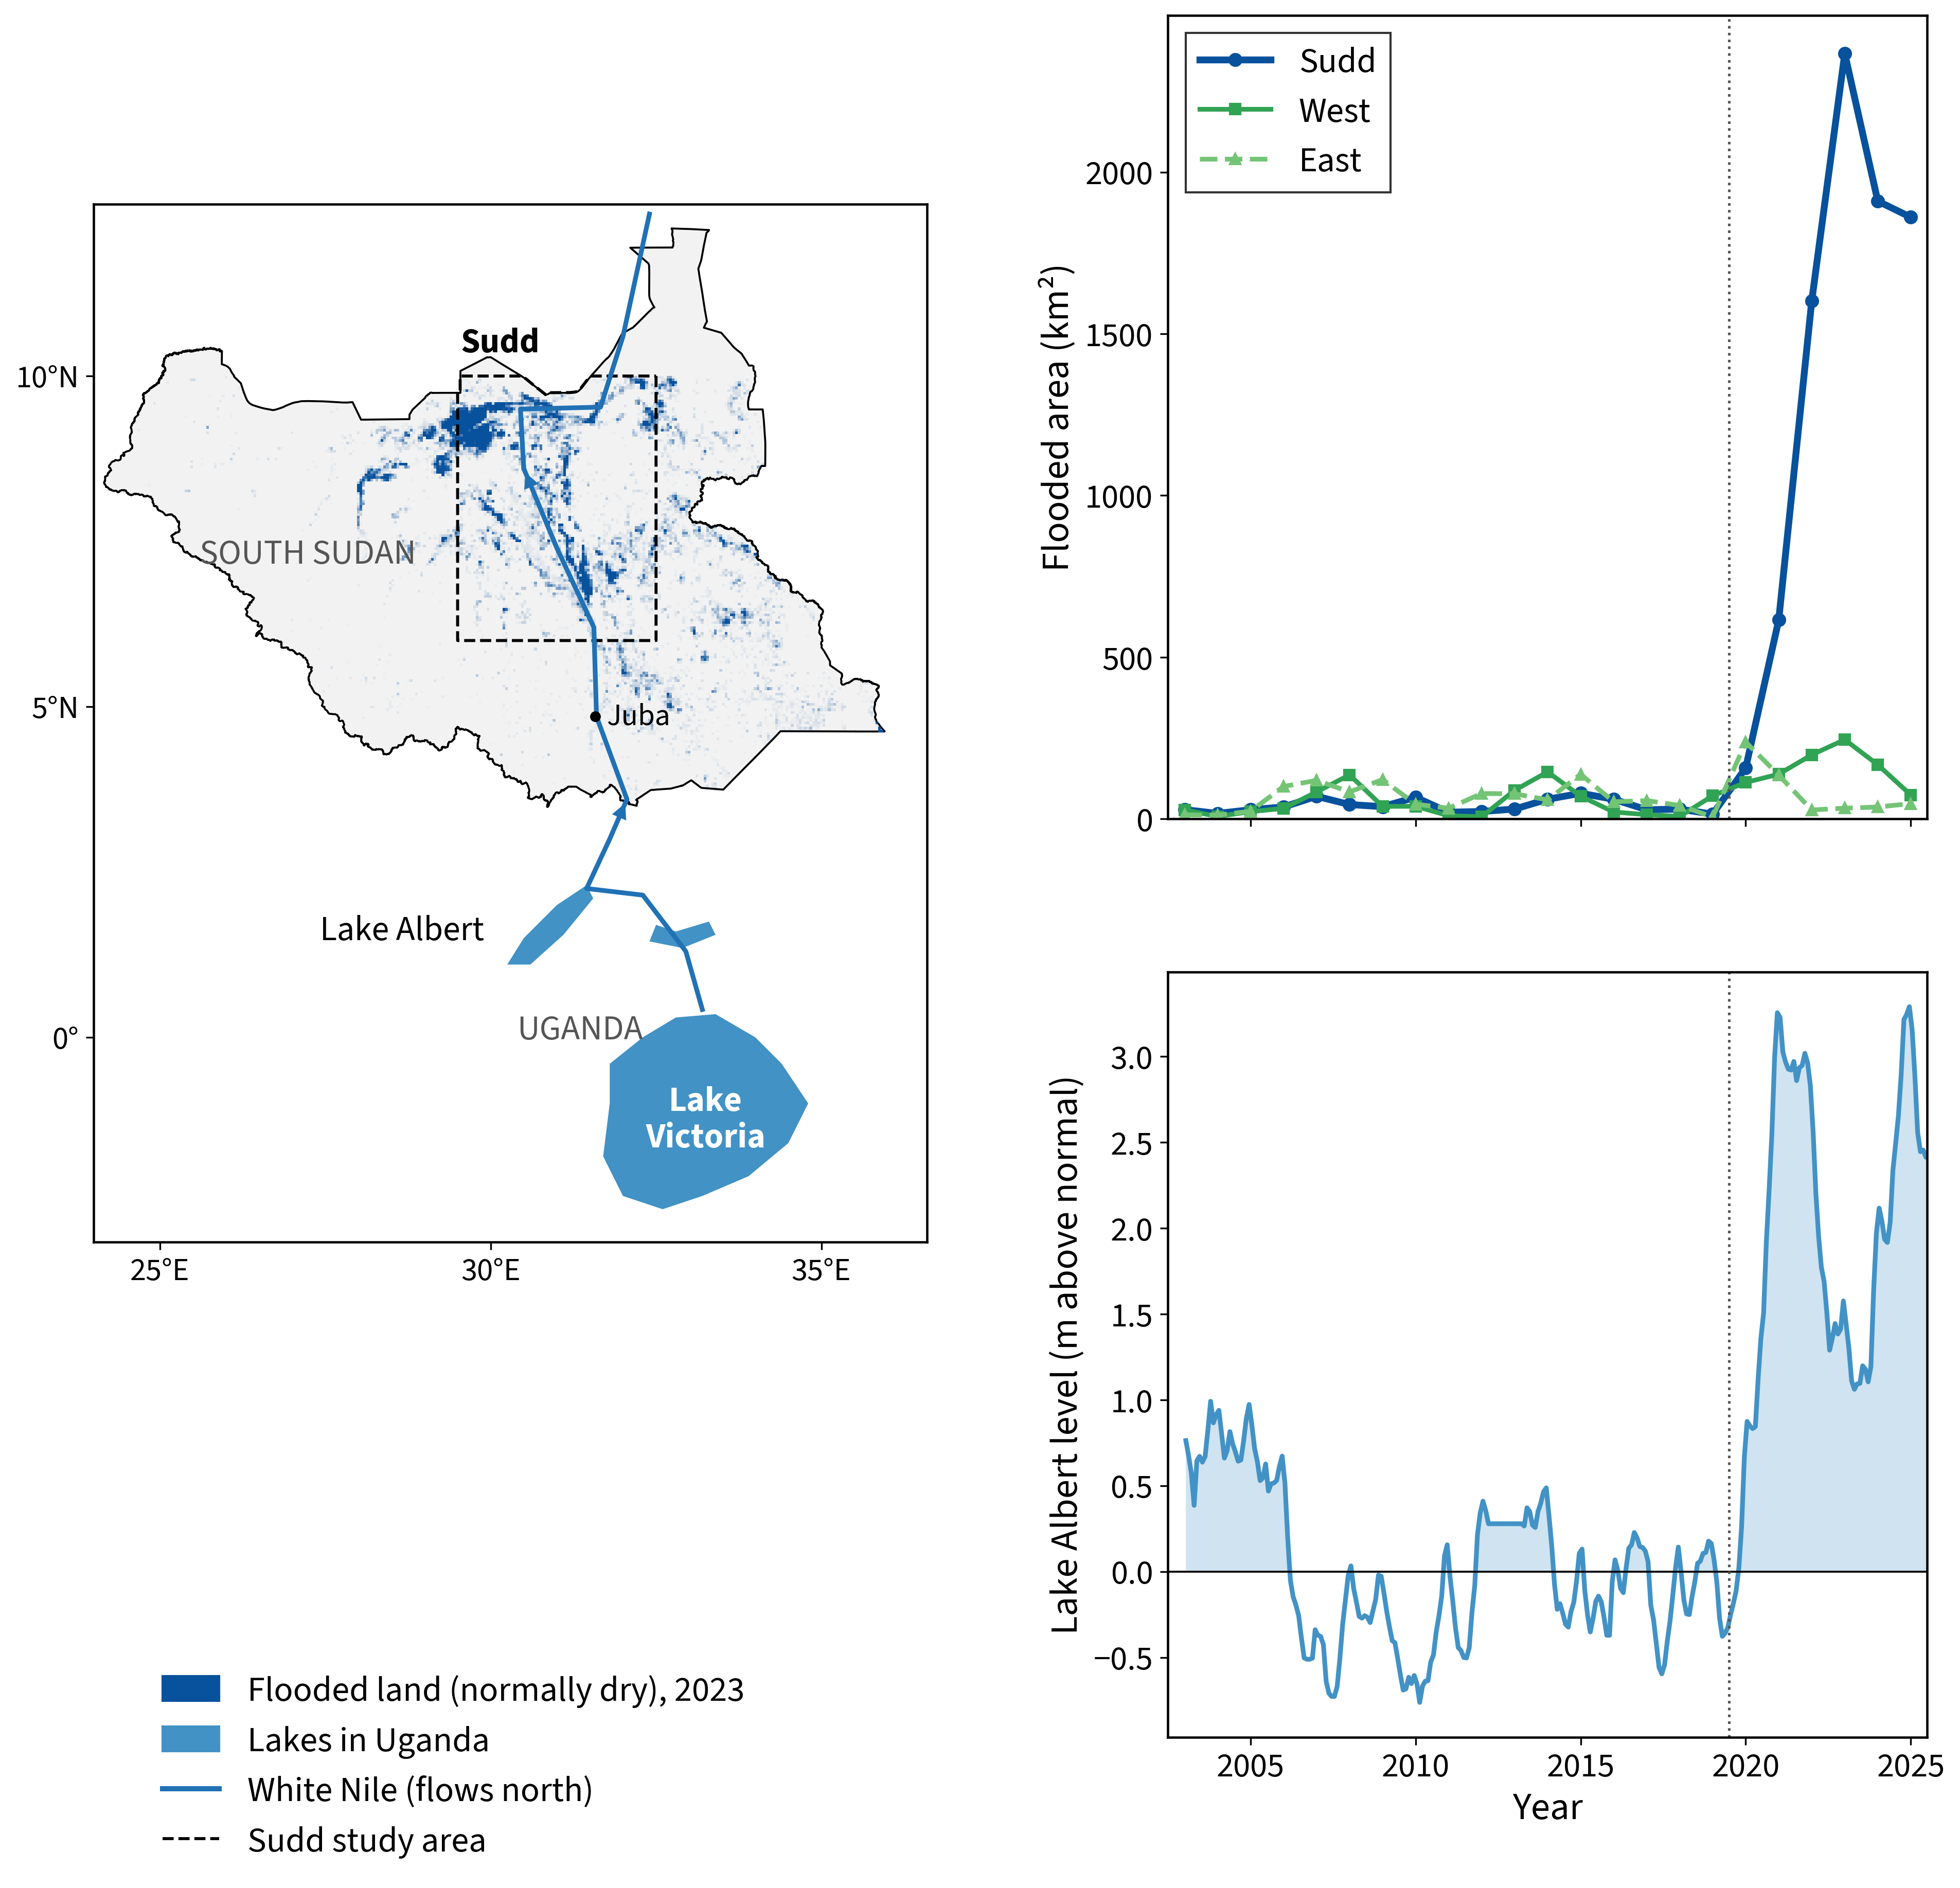
\includegraphics[width=0.74\textwidth]{figures/sq1_combined.png}
\caption{Study area and regime shift. Left: Lakes Victoria and Albert feed the Sudd via the White Nile; blue is normally
dry land flooded in 2023. Right: yearly unusual flood area per region and Lake Albert level.}
\label{fig:context}
\end{figure}

% ---------------------------------------------------------------------------------------------
\section{Research Objective}
The overall question is: \emph{which hydro-climatic drivers are associated with changing flood patterns, and where do
these hazards coincide with high exposure and vulnerability at ADM3 level?} This report covers:

\begin{description}\setlength\itemsep{0pt}
\item[SQ1a] Quantify the factors associated with the shift from seasonal to extreme flooding, as odds ratios with 95\%
confidence intervals.
\item[SQ1b] Test whether upstream water-level anomalies give early indication. This means measuring out-of-sample
skill 4--52 weeks ahead, against local-only information, climatology and persistence.
\item[SQ3] Rank the 512 payams for anticipatory action by combining hazard, exposure and vulnerability.
\end{description}

SQ2 (a random-forest exposure model, by teammates) is used only for comparison.

\textbf{Assumptions limiting scope.}
\begin{itemize}\setlength\itemsep{0pt}
\item An \emph{extreme week} is one in which South Sudan's unusual flood area exceeds the 2003--2019 90th percentile
(408\,km$^2$; Figure~\ref{fig:threshold}).
\item The analysis is weekly and national for SQ1, with ADM3 units for SQ3.
\item Lake Albert represents upstream storage.
\end{itemize}

\textbf{Criteria for an adequate solution.}
\begin{enumerate}\setlength\itemsep{0pt}
\item Skill above climatology and persistence at leads of at least 13 weeks, the window anticipatory financing needs.
\item Interpretable factor effects.
\item Uncertainty that is quantified honestly.
\item Robustness to the definition of ``extreme''.
\item Transparent, reproducible ADM3 outputs.
\end{enumerate}

\begin{figure}[H]
\centering
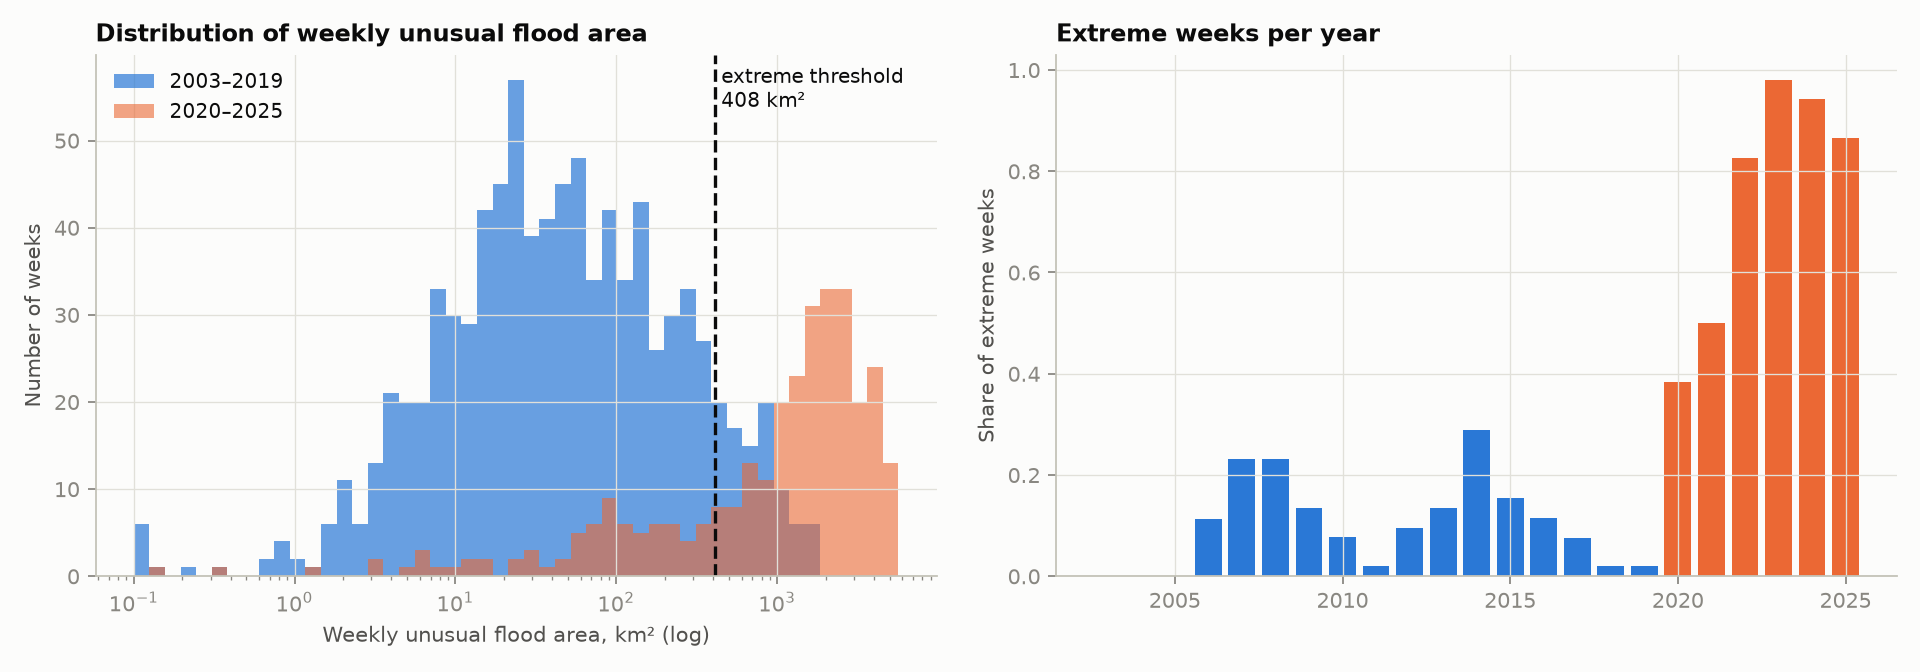
\includegraphics[width=0.82\textwidth]{figures/eda_03_extreme_threshold.png}
\caption{Target definition: weekly unusual flood area with the 408\,km$^2$ threshold (left) and the share of extreme
weeks per year (right).}
\label{fig:threshold}
\end{figure}

% ---------------------------------------------------------------------------------------------
\section{Approach}
Figure~\ref{fig:pipeline} shows the pipeline. All steps run in one reproducible notebook.

\begin{figure}[H]
\centering
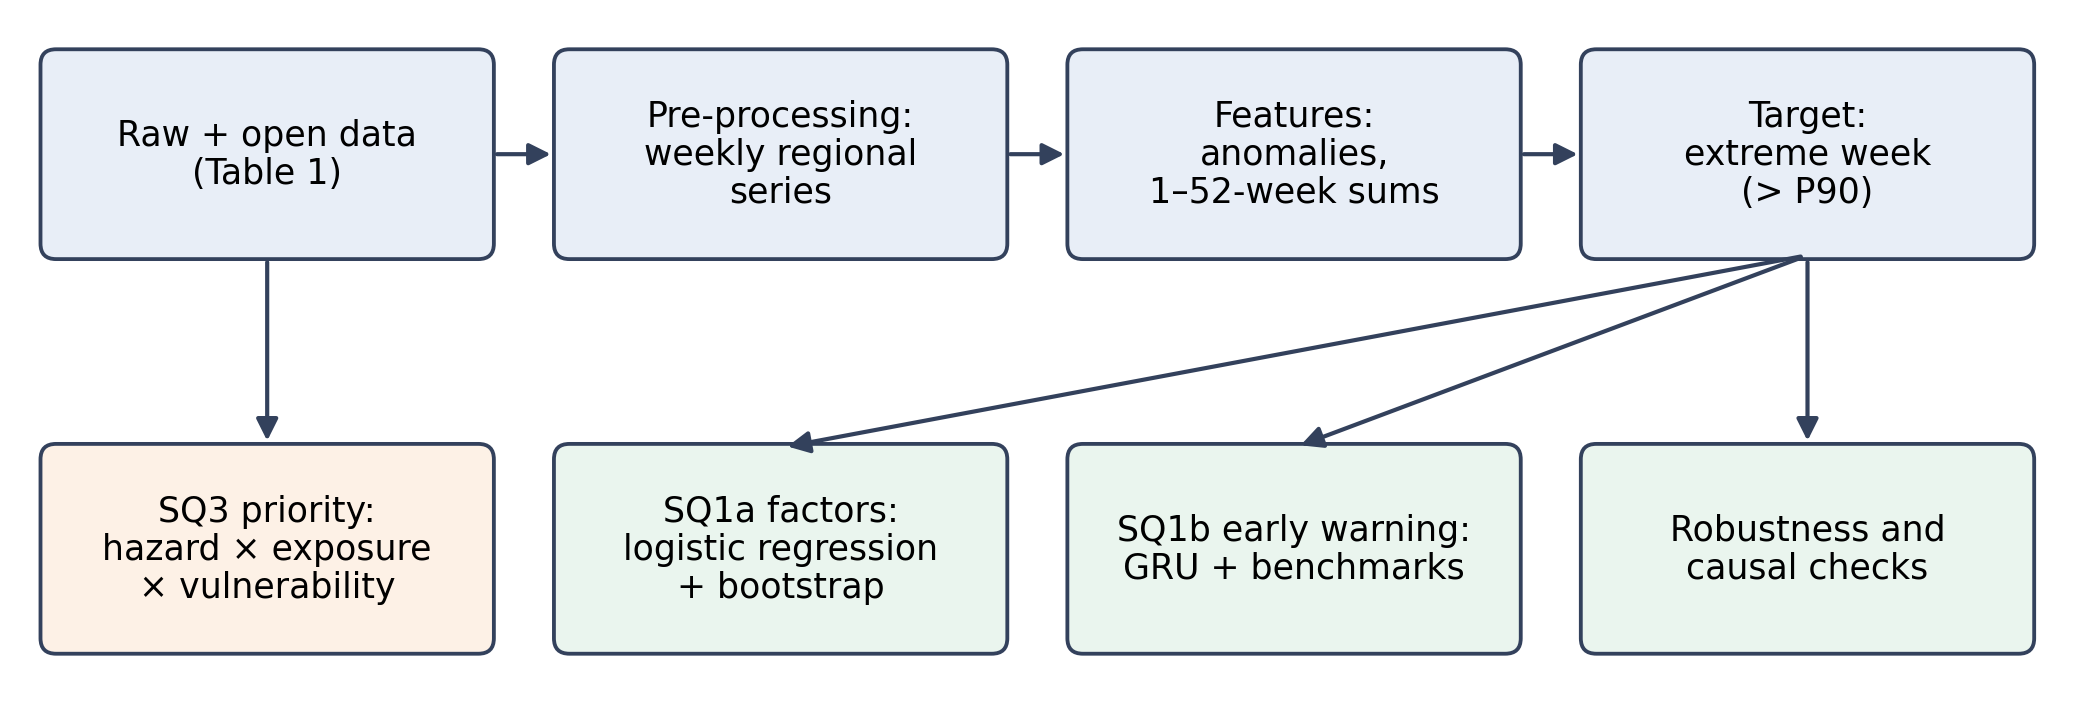
\includegraphics[width=0.9\textwidth]{figures/pipeline.png}
\caption{Analysis pipeline: inputs, processing steps and the three analysis branches.}
\label{fig:pipeline}
\end{figure}

\textbf{Pre-processing.}
\begin{itemize}\setlength\itemsep{0pt}
\item Flood masks are clipped to South Sudan, converted to km$^2$ and aggregated to the weekly maximum of the 3-day
composites, which is robust to cloud gaps.
\item Hourly ERA5 is summed to daily totals and averaged over hydrological regions.
\item Altimetry gaps are filled forward only, so no future information enters a feature.
\end{itemize}

\textbf{Features.} Weekly anomalies relative to the 2003--2019 week-of-year climatology are accumulated over 1--52
weeks. Upstream features include:
\begin{itemize}\setlength\itemsep{0pt}
\item the Lake Albert level and its 26-week rise,
\item the Victoria and Kyoga levels,
\item lake-basin and Sobat rain and runoff,
\item the IOD, lagged one month for availability.
\end{itemize}
Near-duplicate drivers (rain vs rain $-$ evaporation, $r=0.99$) are never combined.

\textbf{SQ1a.} A logistic regression on flood-season weeks (July--December) contrasts extreme with normal seasons, not
wet with dry. It has one driver per physical pathway (all variance inflation factors below 3) and is fitted for
2003--2019 and for 2003--2025.

\textbf{SQ1b.}
\begin{itemize}\setlength\itemsep{0pt}
\item A GRU \cite{cho2014} (32 units, 52-week input window, three seeds averaged) predicts P(extreme) 2--26 weeks
ahead.
\item It is benchmarked against climatology, persistence (current flood state + season), logistic regression,
gradient boosting and an ensemble.
\item Separate logistic models compare upstream-only, local-only and combined information at 4--52 weeks.
\end{itemize}

\textbf{SQ3.} Per payam:
\begin{itemize}\setlength\itemsep{0pt}
\item \textbf{Hazard} is the peak flooded share 2021--25, log-scaled so that 30\% or more scores 1.
\item \textbf{Exposure} is the rank of people and cattle.
\item \textbf{Vulnerability} is the rank of the IPC 3+ share.
\end{itemize}
Priority is their geometric mean, as in INFORM \cite{inform2017}, so it is high only when all three are high.

\textbf{Beyond the state of the art.} Four additions test whether relations reflect the physical pathway, which decides
generalisation beyond 2003--2025:
\begin{itemize}\setlength\itemsep{0pt}
\item a spatial negative control (the Sudd vs regions not downstream of the lakes),
\item a surrogate test against chance alignment,
\item a physically constrained model,
\item validation with independent records (Landsat, G-REALM, documented events, the 1960s).
\end{itemize}

% ---------------------------------------------------------------------------------------------
\section{Evaluation Methodology}
\textbf{Validation schemes.}
\begin{itemize}\setlength\itemsep{0pt}
\item \textbf{Leave-one-year-out (LOYO):} each year is predicted by a model trained on the other years, with a 13-week
buffer.
\item \textbf{Forward test:} train on 2003--2018 and test on 2019--2025, to ask whether the regime shift was
foreseeable.
\end{itemize}

\textbf{Measures.}
\begin{itemize}\setlength\itemsep{0pt}
\item \textbf{ROC-AUC} measures how well a model ranks extreme above normal weeks.
\item \textbf{Brier skill score (BSS)} against climatology measures probabilistic accuracy, which matters because
triggers are set on probabilities.
\end{itemize}

\textbf{Uncertainty.} 95\% intervals, including those for differences between models, come from a bootstrap that
resamples whole years, which respects autocorrelation.

\textbf{Causal plausibility.}
\begin{itemize}\setlength\itemsep{0pt}
\item regional growth factors,
\item local rain during extremes (a competing explanation),
\item partial correlations,
\item lake levels before documented corridor versus western floods.
\end{itemize}
These map onto criteria 1--4.

% ---------------------------------------------------------------------------------------------
\section{Results}
\textbf{Forecast skill.}
\begin{itemize}\setlength\itemsep{0pt}
\item The ensemble reaches AUC 0.96 at 2 weeks and 0.91 at 26 weeks (BSS 0.64 to 0.50; Figure~\ref{fig:skill},
Table~\ref{tab:results}).
\item Persistence is as good at 2--4 weeks. The ensemble is significantly better at 13 weeks (+0.16 BSS,
CI 0.10--0.24) and 26 weeks (+0.27, CI 0.13--0.43).
\item The GRU alone did not beat simpler models.
\item \textbf{Negative result:} every model trained on 2003--2018 missed the persistent 2022--25 extremes
(Figure~\ref{fig:forward}). Even a physically constrained model failed: unconstrained, it learned a negative lake
effect, because the lake was moderately high in 2003--05 without extremes.
\end{itemize}

\begin{figure}[H]
\centering
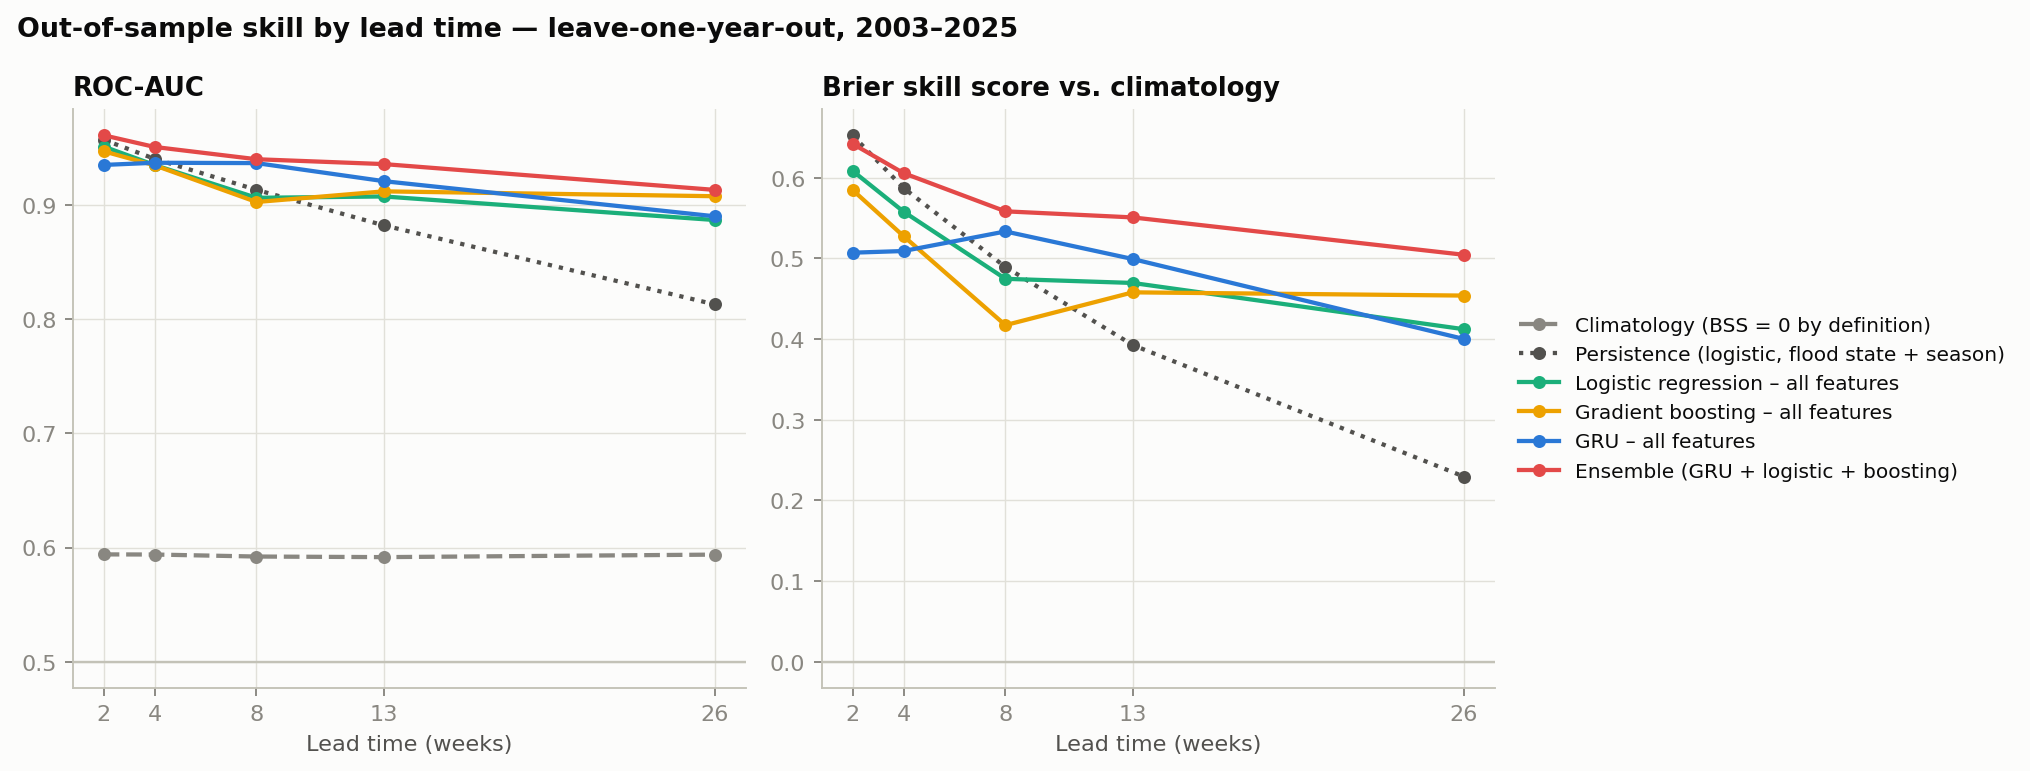
\includegraphics[width=0.9\textwidth]{figures/04a_skill_by_lead_loyo_models.png}
\caption{Leave-one-year-out skill by lead time: ROC-AUC (left) and Brier skill score vs climatology (right).}
\label{fig:skill}
\end{figure}

\begin{figure}[H]
\centering
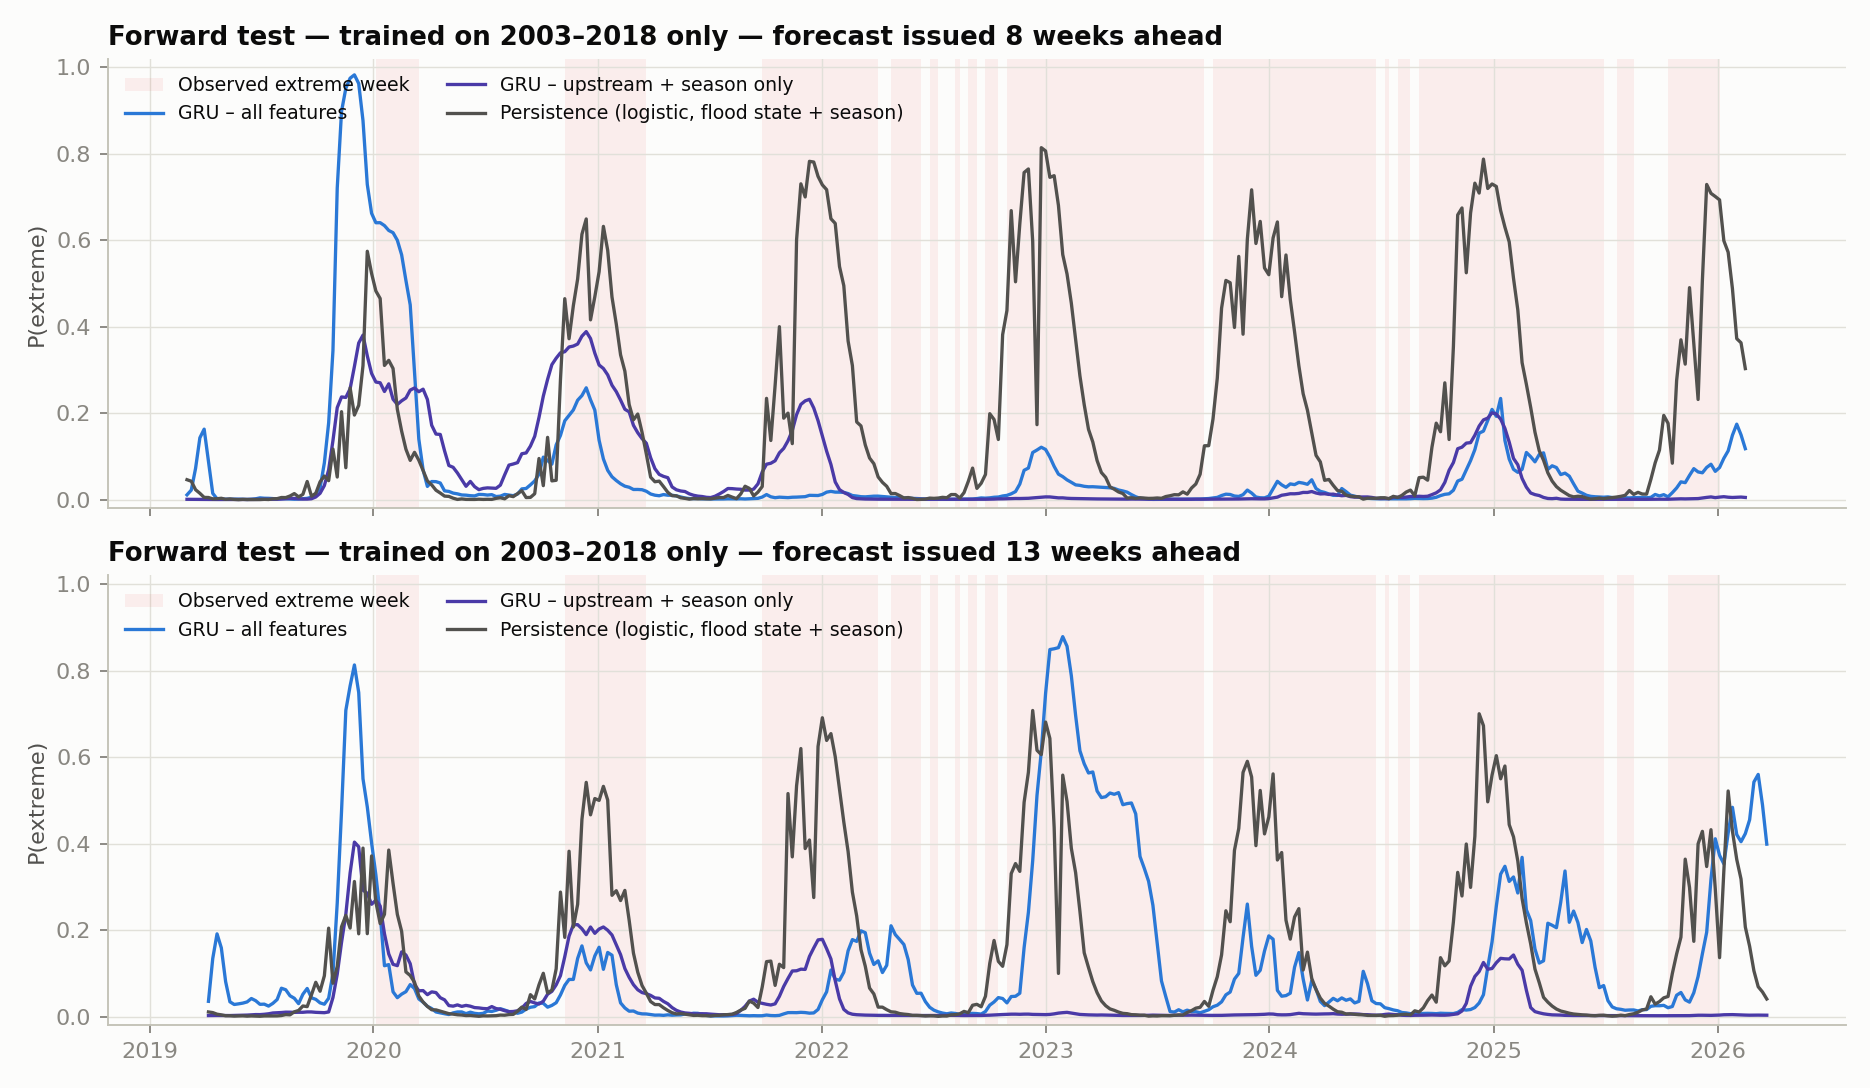
\includegraphics[width=0.78\textwidth]{figures/06_forward_test_2019_2025.png}
\caption{Forward test: models trained on 2003--2018 catch seasonal peaks but miss the year-round extremes (shaded) of
2022--25.}
\label{fig:forward}
\end{figure}

\textbf{Factors (SQ1a; Figure~\ref{fig:odds}).}
\begin{itemize}\setlength\itemsep{0pt}
\item Over 2003--2025, each standard deviation (1.1\,m) of Lake Albert multiplies the odds of an extreme flood season
by 3.8 (CI 2.2--10.3).
\item Recent local rain lowers the odds (0.52, CI 0.30--0.68): floods peak after the rain.
\item Before 2019, with only 44 extreme weeks, no driver is significant in the multivariable model. Univariately,
Sobat rain warns 13 weeks ahead (AUC 0.73, CI 0.60--0.83) and Lake Albert does not.
\end{itemize}

\begin{figure}[H]
\centering
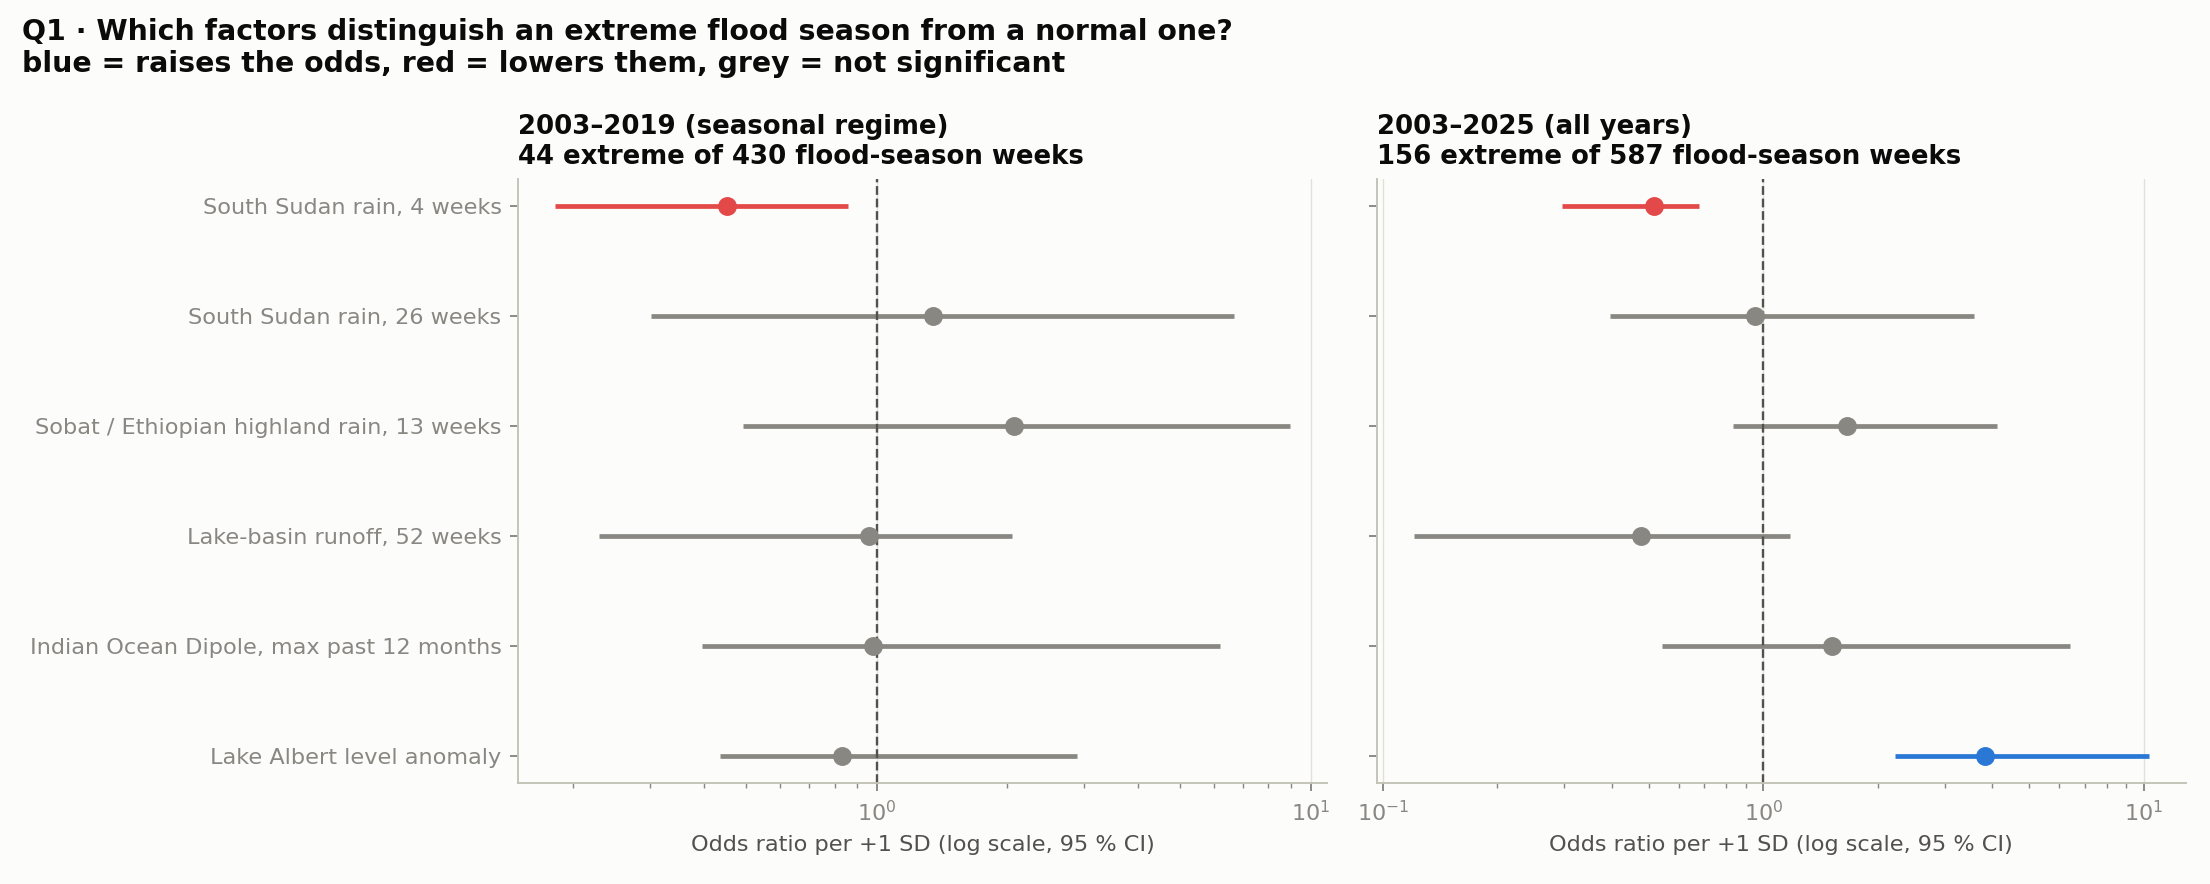
\includegraphics[width=0.9\textwidth]{figures/15_q1_factor_odds_ratios.png}
\caption{Odds ratios per standard deviation with 95\% year-block bootstrap intervals, for 2003--2019 and 2003--2025.}
\label{fig:odds}
\end{figure}

\textbf{Spatial and causal checks (Figure~\ref{fig:spatial}).}
\begin{itemize}\setlength\itemsep{0pt}
\item Unusual flooding grew 36.5$\times$ (CI 21--57) in the Sudd, but only 3.2$\times$ in the west and 0.8$\times$
in the east, neither of which is downstream.
\item Local rain was $-$2.6$\sigma$ during the 2020s extremes.
\item Lake Albert stays associated with Sudd flooding after controlling for lake-basin runoff (partial $r$ 0.54).
\item The results hold for alternative targets (Lake Albert AUC 0.75--0.79 at 26 weeks).
\item Documented corridor floods followed higher Lake Victoria levels than western floods (exact $p=0.036$).
\item The three strongest IOD years (1997, 2019, 2023) were each followed by a lake rise.
\end{itemize}

\begin{figure}[H]
\centering
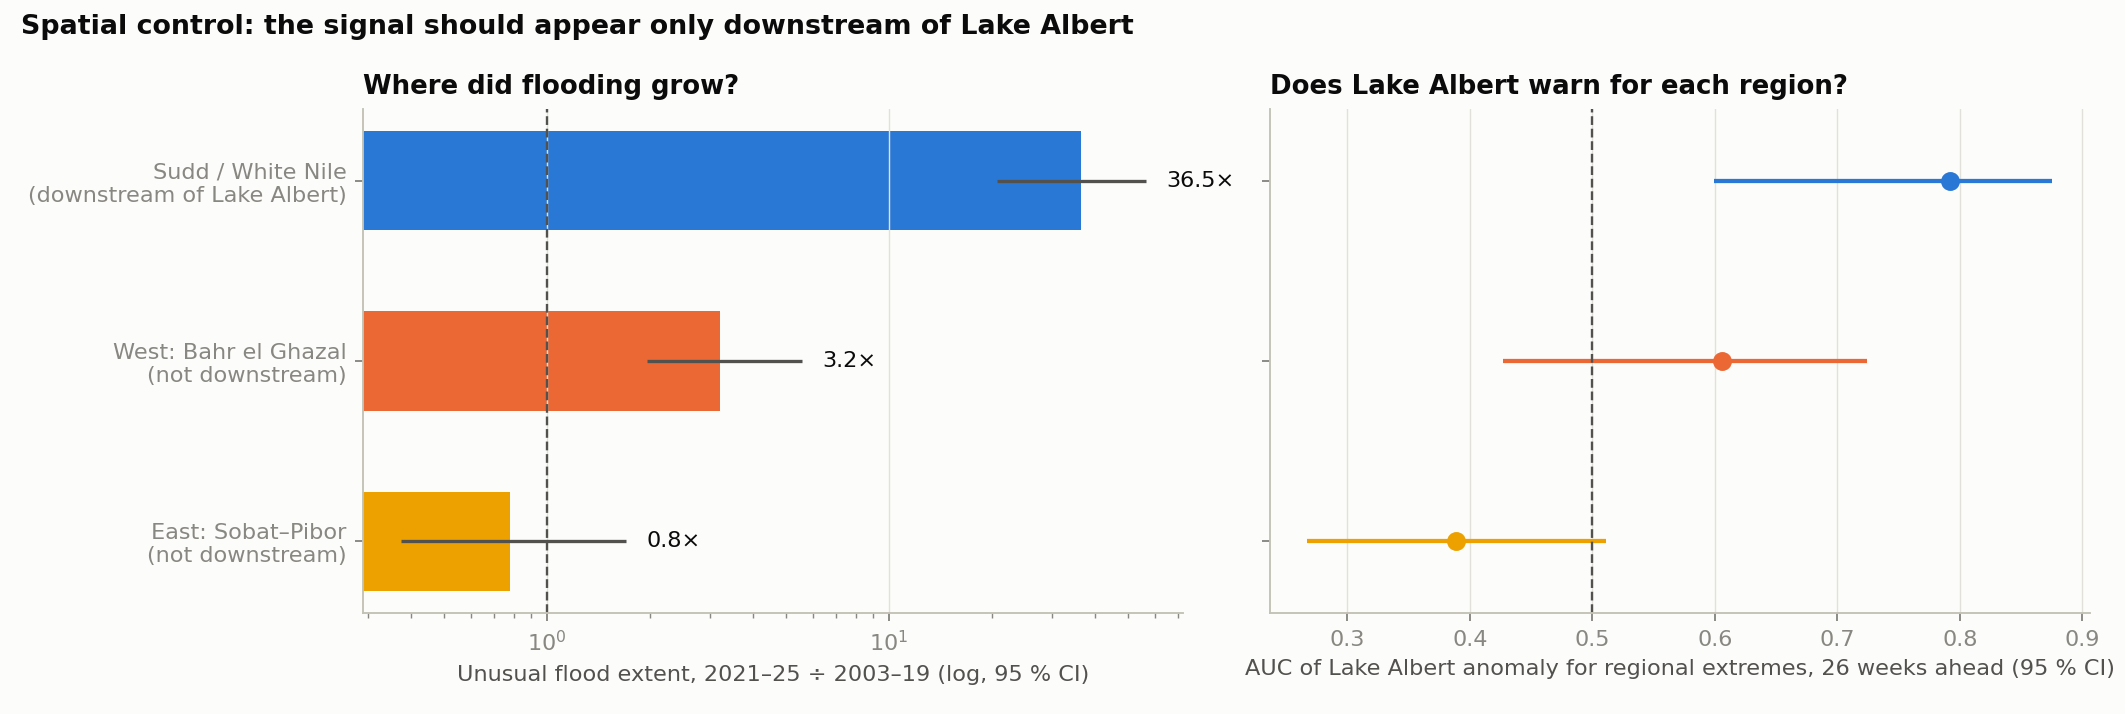
\includegraphics[width=0.82\textwidth]{figures/12_spatial_negative_control.png}
\caption{Spatial control: growth of unusual flooding per region (left) and Lake Albert AUC for regional extremes
(right).}
\label{fig:spatial}
\end{figure}

\textbf{Early indication (SQ1b; Figure~\ref{fig:q2}).}
\begin{itemize}\setlength\itemsep{0pt}
\item Upstream-only models reach AUC 0.81--0.85 up to 52 weeks ahead, against 0.74--0.78 for local-only. The
difference is significant at 13 weeks (+0.19 BSS) and 52 weeks (+0.21).
\item Upstream data add no significant skill beyond persistence.
\item The Lake Albert signal cannot be separated from a simple time trend (AUC 0.82 vs 0.84).
\end{itemize}

\begin{figure}[H]
\centering
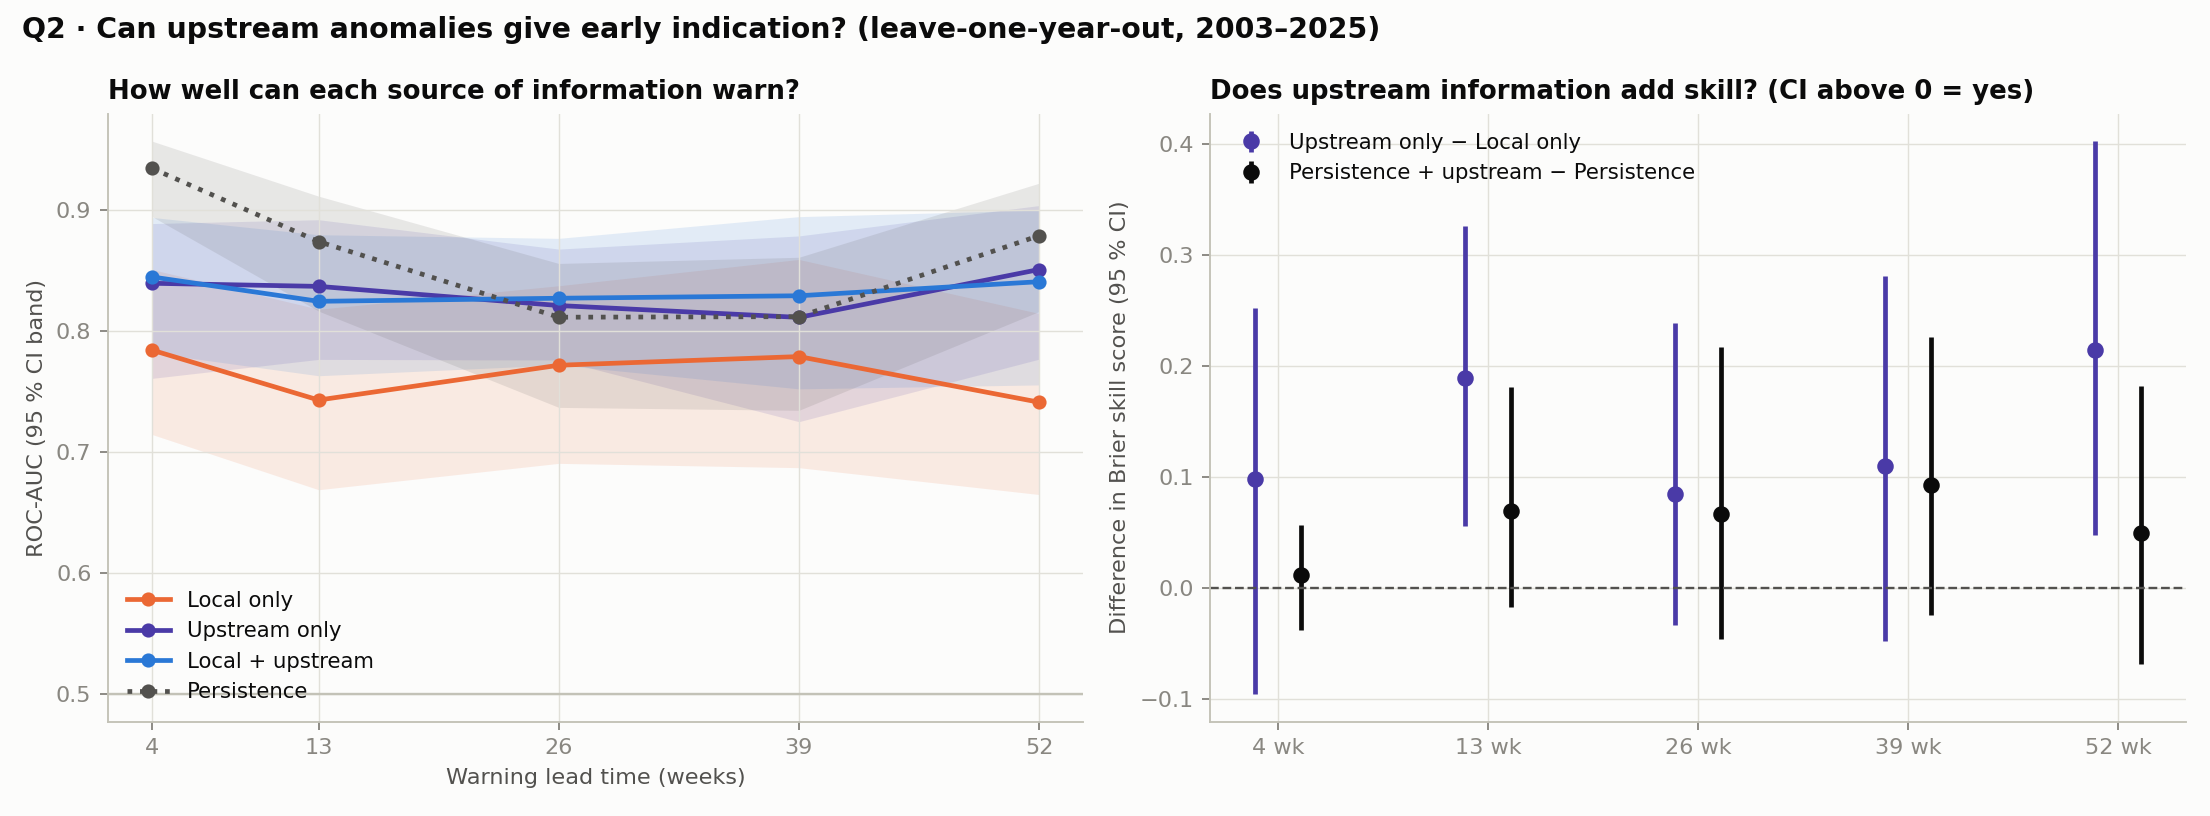
\includegraphics[width=0.9\textwidth]{figures/16_q2_upstream_early_warning.png}
\caption{Early-warning skill by information source (left) and the added skill of upstream data, with 95\% intervals
(right).}
\label{fig:q2}
\end{figure}

\textbf{Prioritisation (SQ3; Figure~\ref{fig:sq3}).}
\begin{itemize}\setlength\itemsep{0pt}
\item The top 10\% (51 payams, 1.7 million people) concentrate in Rubkona (Unity) and in Fangak, Ayod, Duk, Twic East
and Uror (Jonglei).
\item This matches the high-risk zones of the SQ2 random forest (hold-out ROC-AUC 0.88).
\end{itemize}

\begin{table}[H]
\centering\small
\caption{Main quantitative results (95\% confidence intervals in brackets).}
\label{tab:results}
\begin{tabular}{@{}ll@{}}
\toprule
Result & Value\\
\midrule
Ensemble ROC-AUC, 2 / 13 / 26 weeks (LOYO) & 0.96 / 0.94 / 0.91\\
Ensemble $-$ persistence BSS, 13 / 26 weeks & +0.16 [0.10, 0.24] / +0.27 [0.13, 0.43]\\
Forward test, upstream-only AUC at 13 weeks & 0.52\\
Lake Albert odds ratio per SD (2003--2025) & 3.8 [2.2, 10.3]\\
Unusual flooding growth: Sudd / west / east & 36.5$\times$ / 3.2$\times$ / 0.8$\times$\\
Upstream-only vs local-only, BSS gain at 13 / 52 weeks & +0.19 [0.06, 0.33] / +0.21 [0.05, 0.40]\\
Highest-priority payams (SQ3) & 51 payams, 1.7 million people\\
\bottomrule
\end{tabular}
\end{table}

\begin{figure}[H]
\centering
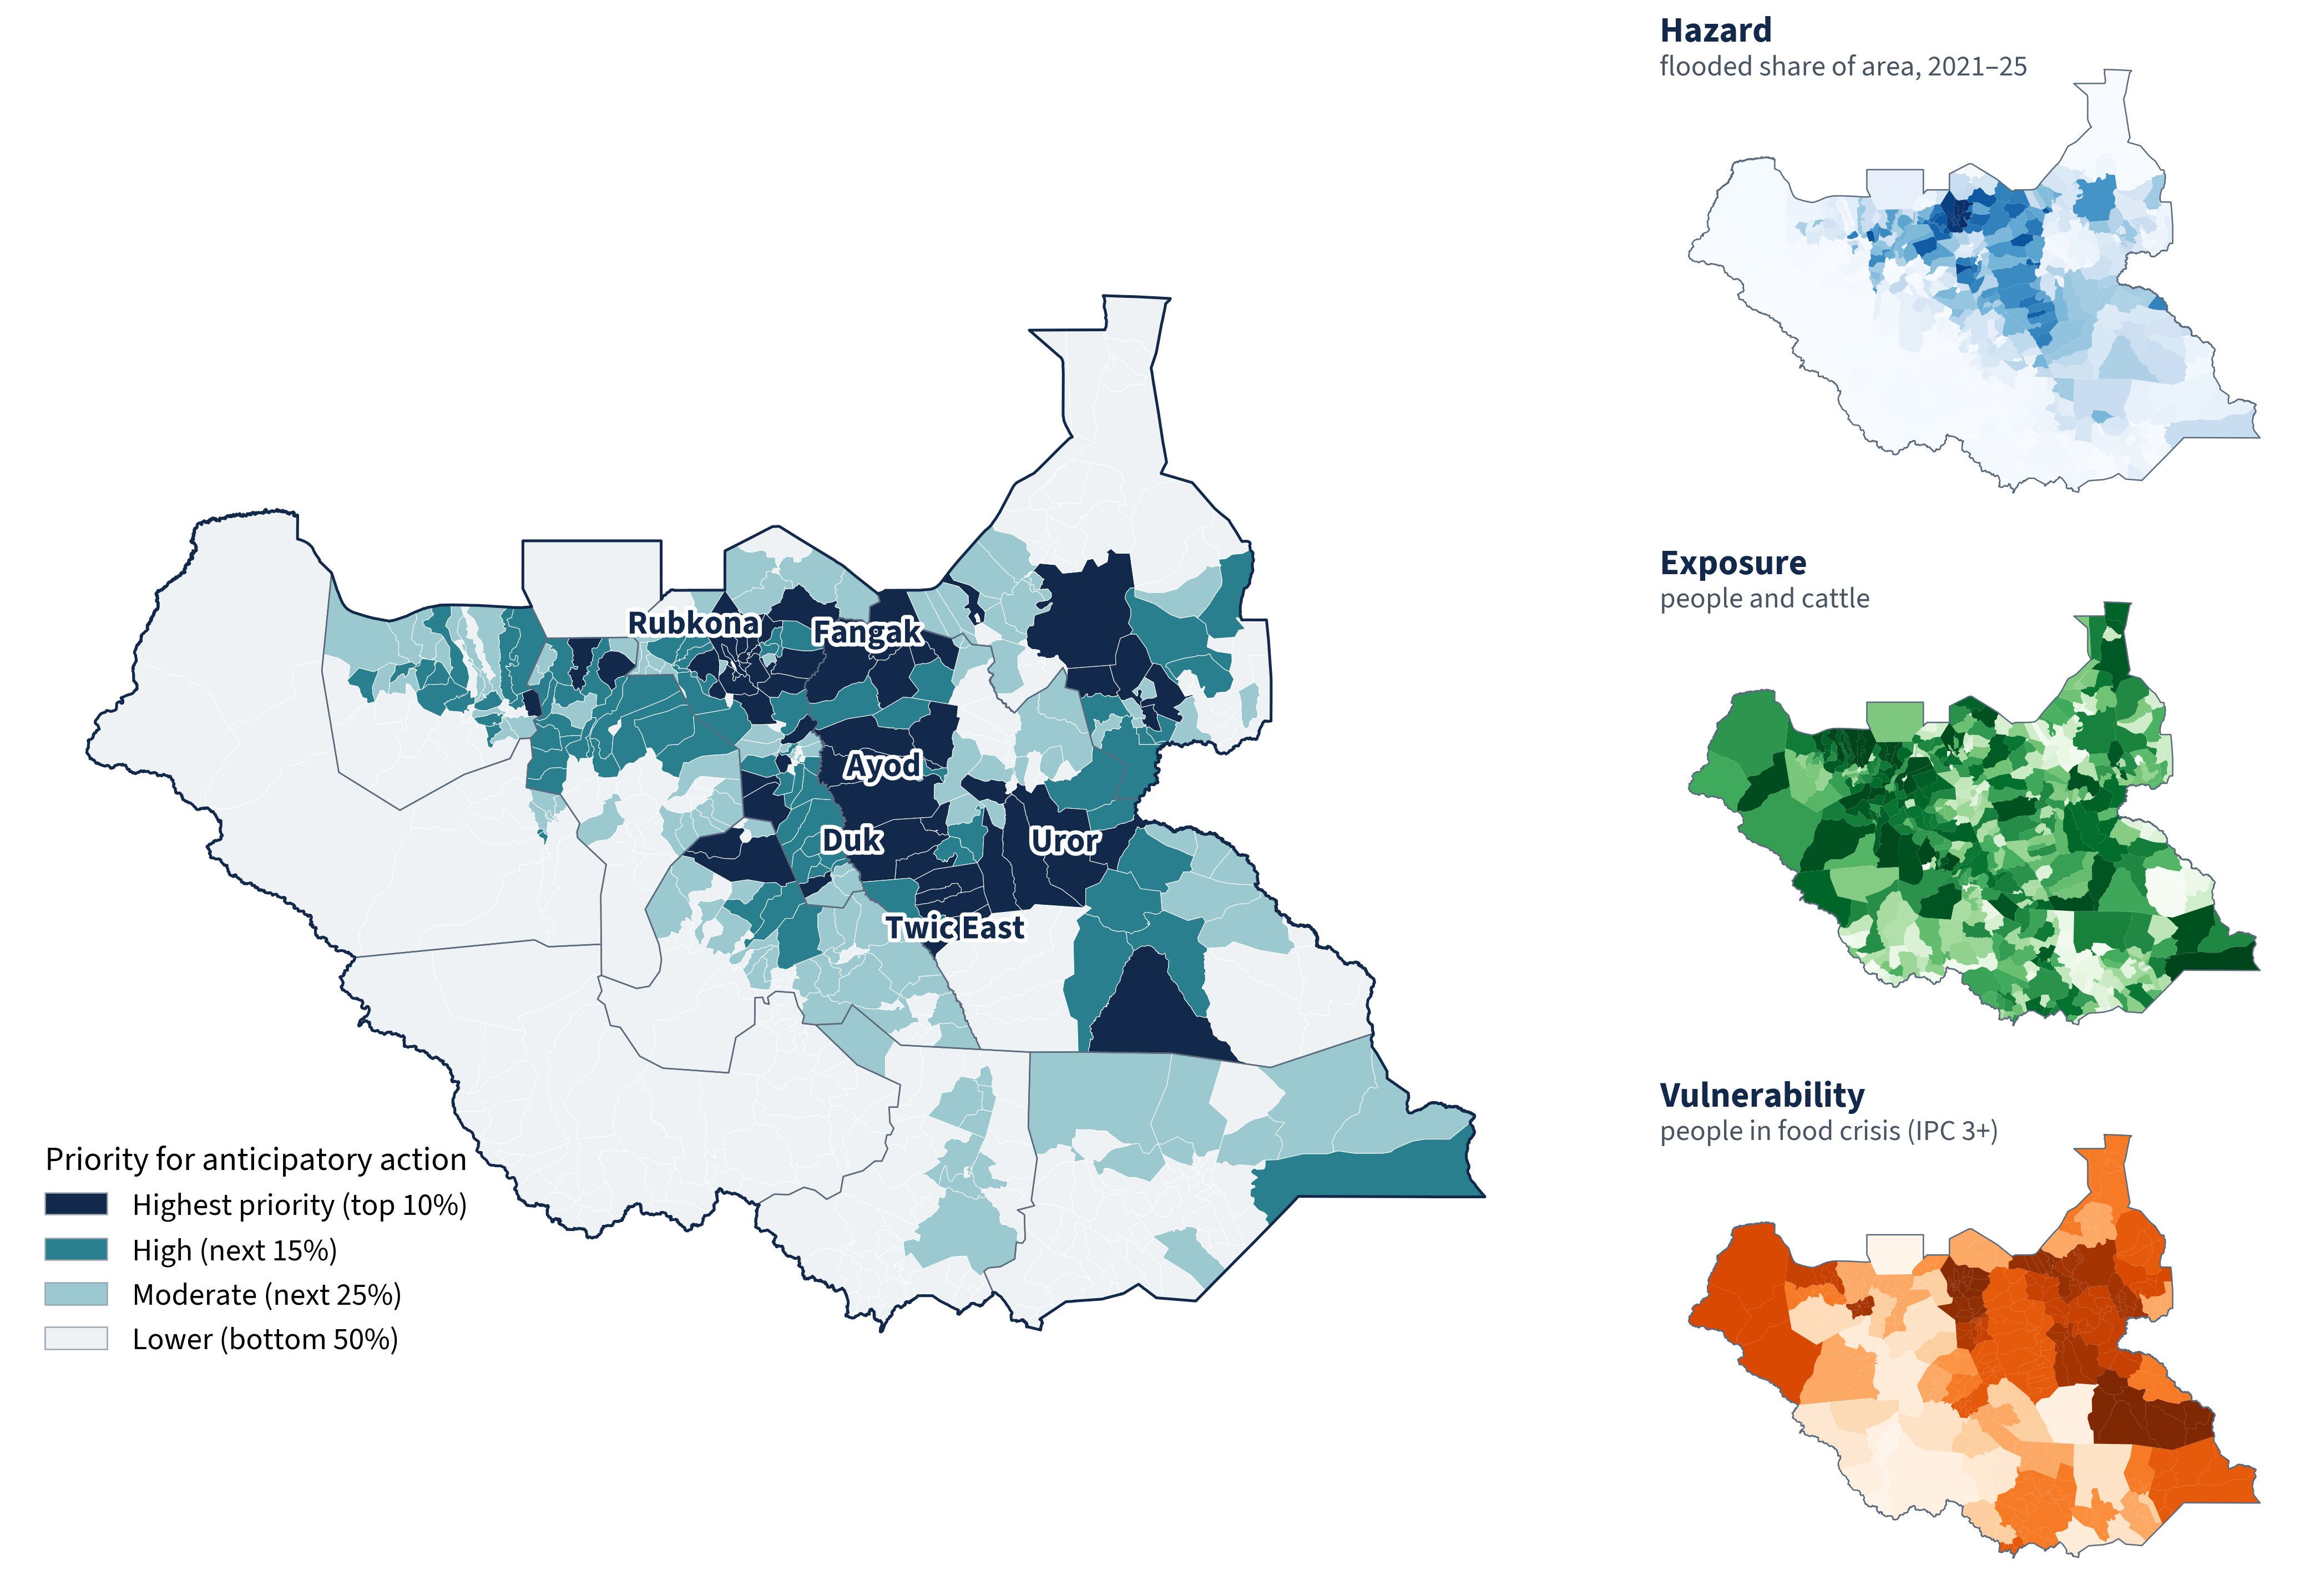
\includegraphics[width=0.78\textwidth]{figures/sq3_priority_map.png}
\caption{ADM3 priority for anticipatory action (left), built from hazard, exposure and vulnerability (right).}
\label{fig:sq3}
\end{figure}

% ---------------------------------------------------------------------------------------------
\section{Discussion}
\textbf{Two regimes.} Before 2020, extremes were seasonal peaks after Ethiopian-highland rain. Since 2020 they are
persistent and confined to the White Nile corridor, coinciding with extreme lake levels while local rain was below
normal. Three findings \emph{support}, but do not prove, the pathway lake outflow $\rightarrow$ Sudd:
\begin{itemize}\setlength\itemsep{0pt}
\item the spatial specificity,
\item the closed local-rain path,
\item the 1960s replication \cite{sutcliffe2018}.
\end{itemize}
The satellite era holds a single above-threshold lake event, and the moderate highs of 1998--2005 caused no expansion,
which suggests a threshold. This explains the main negative result: no model can learn a regime absent from its
training data.

\textbf{Strengths.} Strict evaluation: whole-year resampling, a forward test and reported non-significant gains.

\textbf{Weaknesses and assumptions.}
\begin{itemize}\setlength\itemsep{0pt}
\item Flood masks under-detect vegetated swamp.
\item The P90 threshold and the 2003--2019 reference are choices, although the results held for alternative targets.
\item IPC data exist only per county.
\item The equal SQ3 weights are a value judgement.
\item Persistence dominates short leads, limiting the GRU's value.
\end{itemize}

\textbf{Fulfilment of the objective.} The objective was largely met. SQ1a and SQ3 are answered with quantified
uncertainty, and SQ1b only partly: upstream anomalies are the best long-lead indicator, but not a validated
stand-alone predictor.

\textbf{Impact.} Monitoring the lakes could extend warning windows to months. The risks are overconfidence from one
event, and deprioritising areas that are poorly measured.

% ---------------------------------------------------------------------------------------------
\section{Conclusion}
In 2020, extreme flooding in South Sudan shifted from rain-driven seasonal peaks to persistent, lake-driven inundation
of the Sudd. Upstream lake anomalies are the most promising early indicator, but they rest on few events.

\textbf{Recommendations to WFP and partners.}
\begin{enumerate}\setlength\itemsep{0pt}
\item Add Lake Albert and Victoria levels and the September--November IOD to early-warning monitoring. Validate Lake
Albert above +1\,m as a trigger prospectively: it was exceeded on only 2 weeks in 2003--18 and preceded the 2020
regime by 13 weeks.
\item Use the ensemble for 13--26-week outlooks and persistence for shorter leads.
\item Pre-position support in Rubkona and central Jonglei, scaling action to data confidence instead of skipping
poorly measured payams.
\item Keep human sign-off on triggers and publish the SQ3 weights and their sensitivity.
\end{enumerate}

\textbf{Further research.}
\begin{itemize}\setlength\itemsep{0pt}
\item Hydrological routing of lake releases.
\item Radar flood data.
\item Payam-level vulnerability data.
\item Re-evaluation after each flood season.
\end{itemize}

\small
\begin{thebibliography}{9}\setlength\itemsep{0pt}
\bibitem{cho2014} Cho, K. et al. (2014). Learning phrase representations using RNN encoder--decoder for statistical machine translation. \emph{EMNLP}, 1724--1734.
\bibitem{hersbach2020} Hersbach, H. et al. (2020). The ERA5 global reanalysis. \emph{Q. J. R. Meteorol. Soc.}, 146, 1999--2049.
\bibitem{inform2017} Marin-Ferrer, M., Vernaccini, L., \& Poljansek, K. (2017). \emph{INFORM Index for Risk Management: Concept and Methodology}. JRC, EUR 28655.
\bibitem{pekel2016} Pekel, J.-F. et al. (2016). High-resolution mapping of global surface water and its long-term changes. \emph{Nature}, 540, 418--422.
\bibitem{saji1999} Saji, N. H. et al. (1999). A dipole mode in the tropical Indian Ocean. \emph{Nature}, 401, 360--363.
\bibitem{sutcliffe2018} Sutcliffe, J. V., \& Brown, E. (2018). Water losses from the Sudd. \emph{Hydrol. Sci. J.}, 63(4), 527--541.
\bibitem{sutcliffe1999} Sutcliffe, J. V., \& Parks, Y. P. (1999). \emph{The Hydrology of the Nile}. IAHS Special Publication 5.
\end{thebibliography}

\end{document}
